% !TEX root = main.tex
\chapter{RESULTS AND DISCUSSIONS}
\section{General Trends}
\subsection{Grab Sample}
In our analysis of MC, MC-RR, MC-LR and MC-LA were the most detected congeners throughout the summer.  MC-RR was found with the highest concentrations 8.55 $\mu$g/L at Brighton Lake in August (see figure \ref{fig:month}).  Majority of our samples were below the EPA guidance level. From our sampled lake sites, Belleville, Brighton, Ford, Hudson, and Wixom Lake had instances of MC concentrations that exceeded the EPA guidance level of 4 $\mu$g/L both from \gls{lcmsms} and ELISA analysis (see figure \ref{fig:microcystin}).

Of all the sampled lakes, we did not detect any cylindrospermonsin in our surveyed lakes. Moreover,  QPCR analysis did detect genes responsible for producing cylindrospermonsin (\emph{cyrA}) and saxitoxin (\emph{sxtA}). We detected varying amounts of \emph{mcyE} gene copies in each lake.  From the \gls{lcmsms} we found one instance of anatoxin-a detected at Brighton lake in August 2017 which was sampled during an visible bloom (2.80 $\mu$g/L of Anantoxin-a).

\subsection{SPATT}

From the deployed SPATT, MC-LA, MC-LR, and MC-RR were the most frequently detected congener (see \ref{tab:spattcongener}). Microcystin concentrations from SPATT was mostly detected in lake Paradise, Intermediate Lake, Lake Cadillac and Wixom Lake. 


\begin{sidewaysfigure}[!h] 
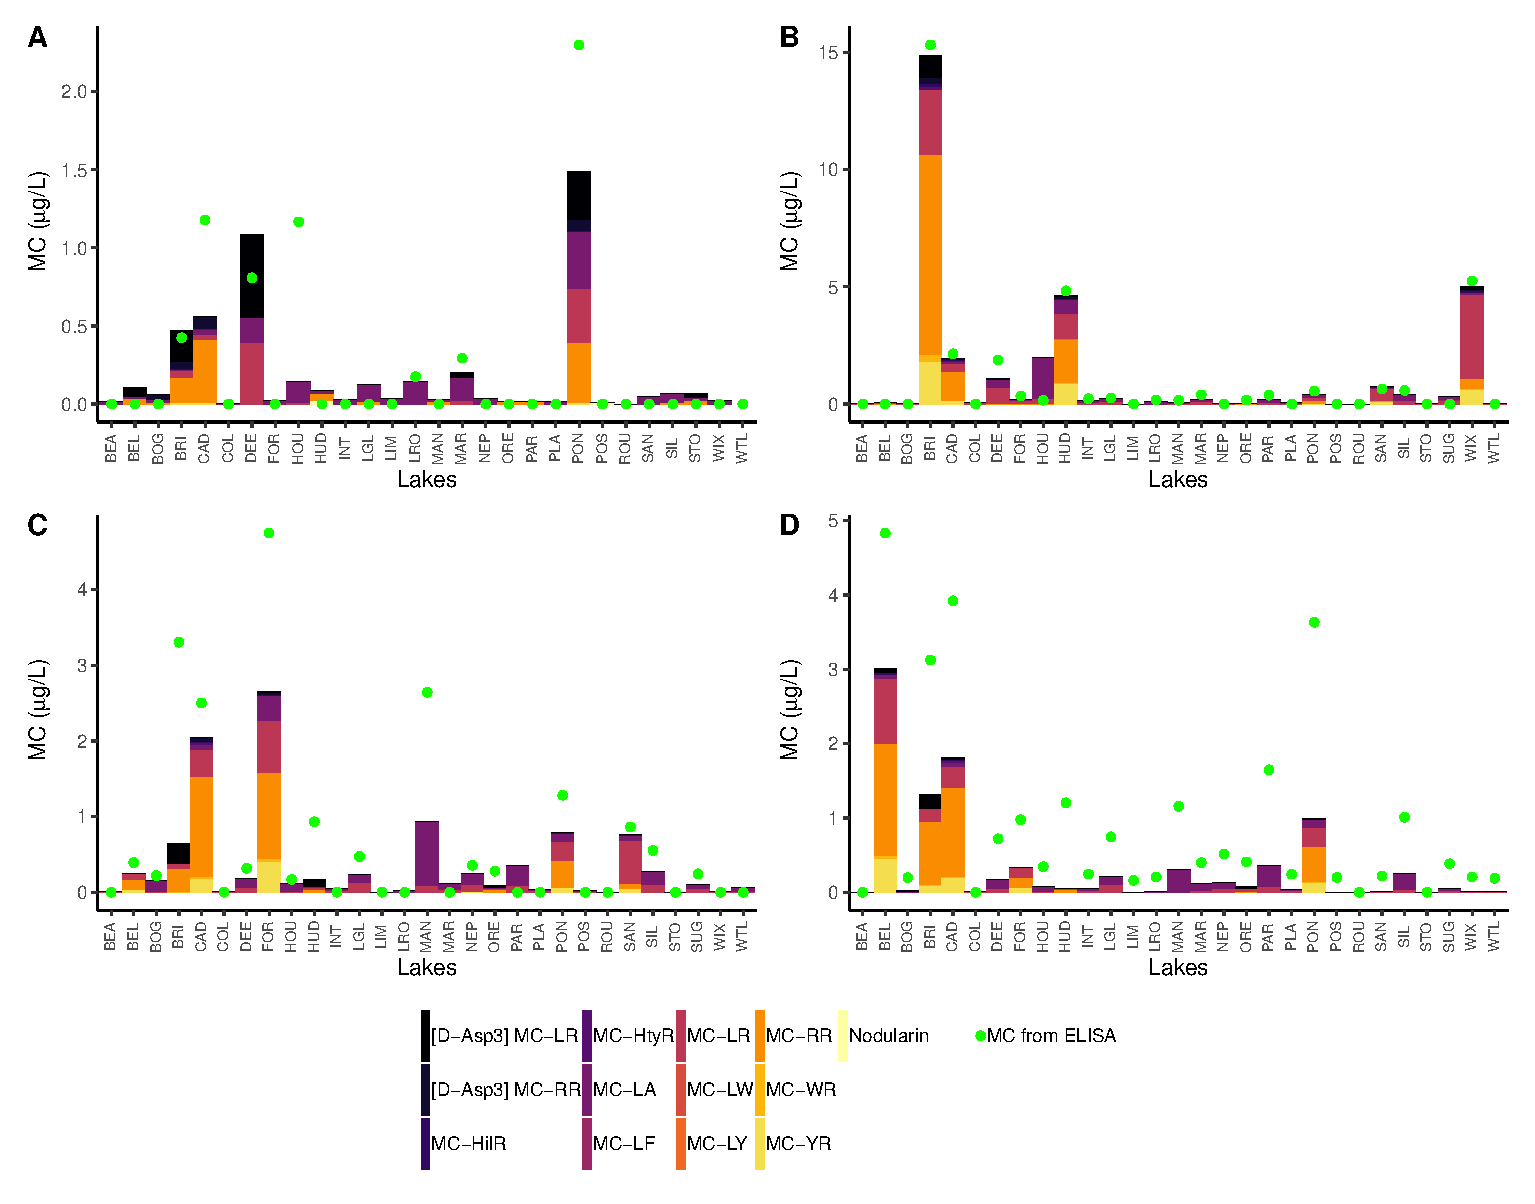
\includegraphics[width=\textwidth]{figures/month}
\caption{
Barplots of MC and their congeners analyzed by LC-MS/MS from grab sample for each lake for the month of 
(A): July, 
(B): August,
(C): September, and
(D): October 
}
\label{fig:month} 
\end{sidewaysfigure}

%EPA Graph
\begin{figure}[!h]
 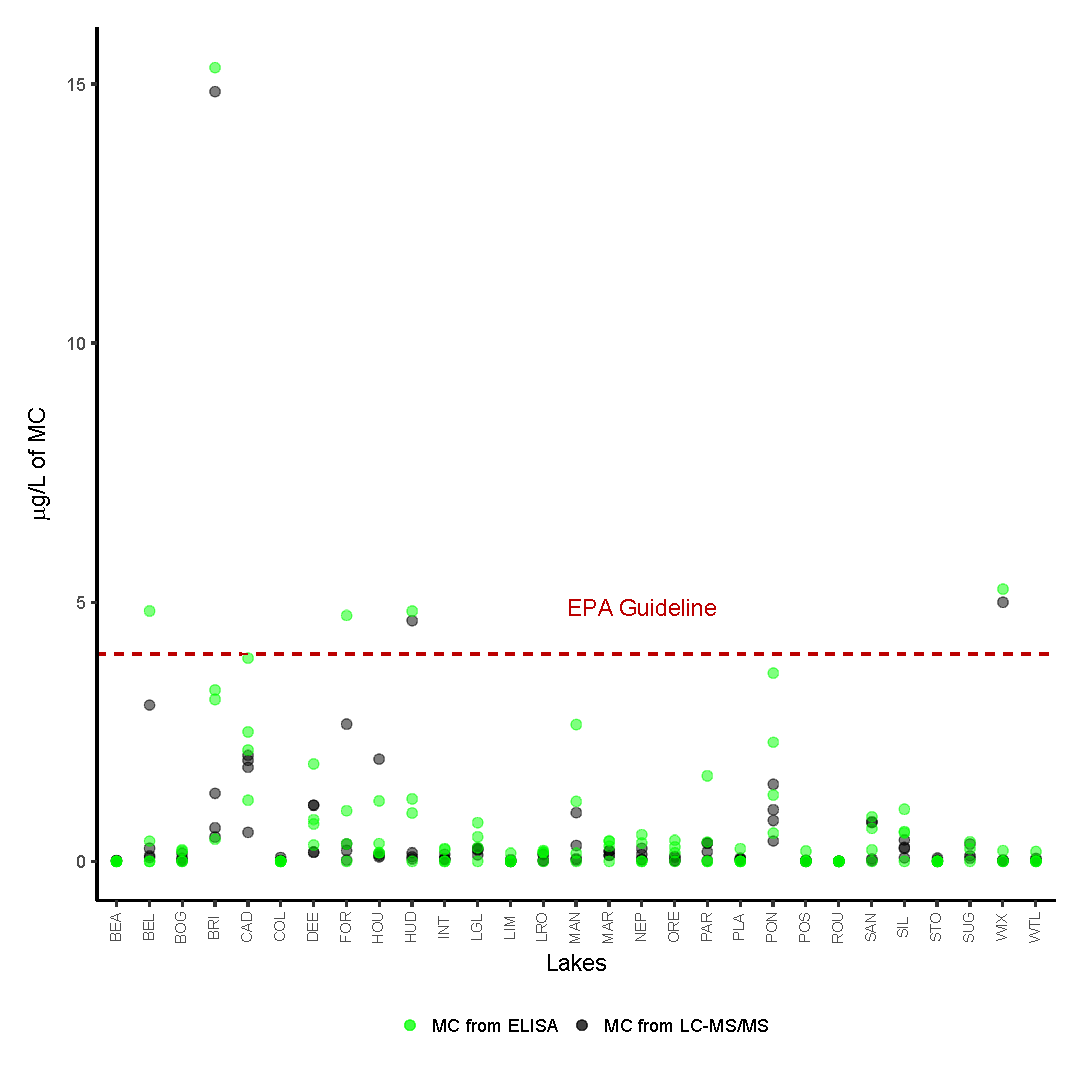
\includegraphics[width=\textwidth]{figures/Microcystin}
 \caption{Total MC with all results from ELISA and LC-MS/MS plotted by each lake}
 \label{fig:microcystin}
\end{figure}


\begin{figure}[!h] 
	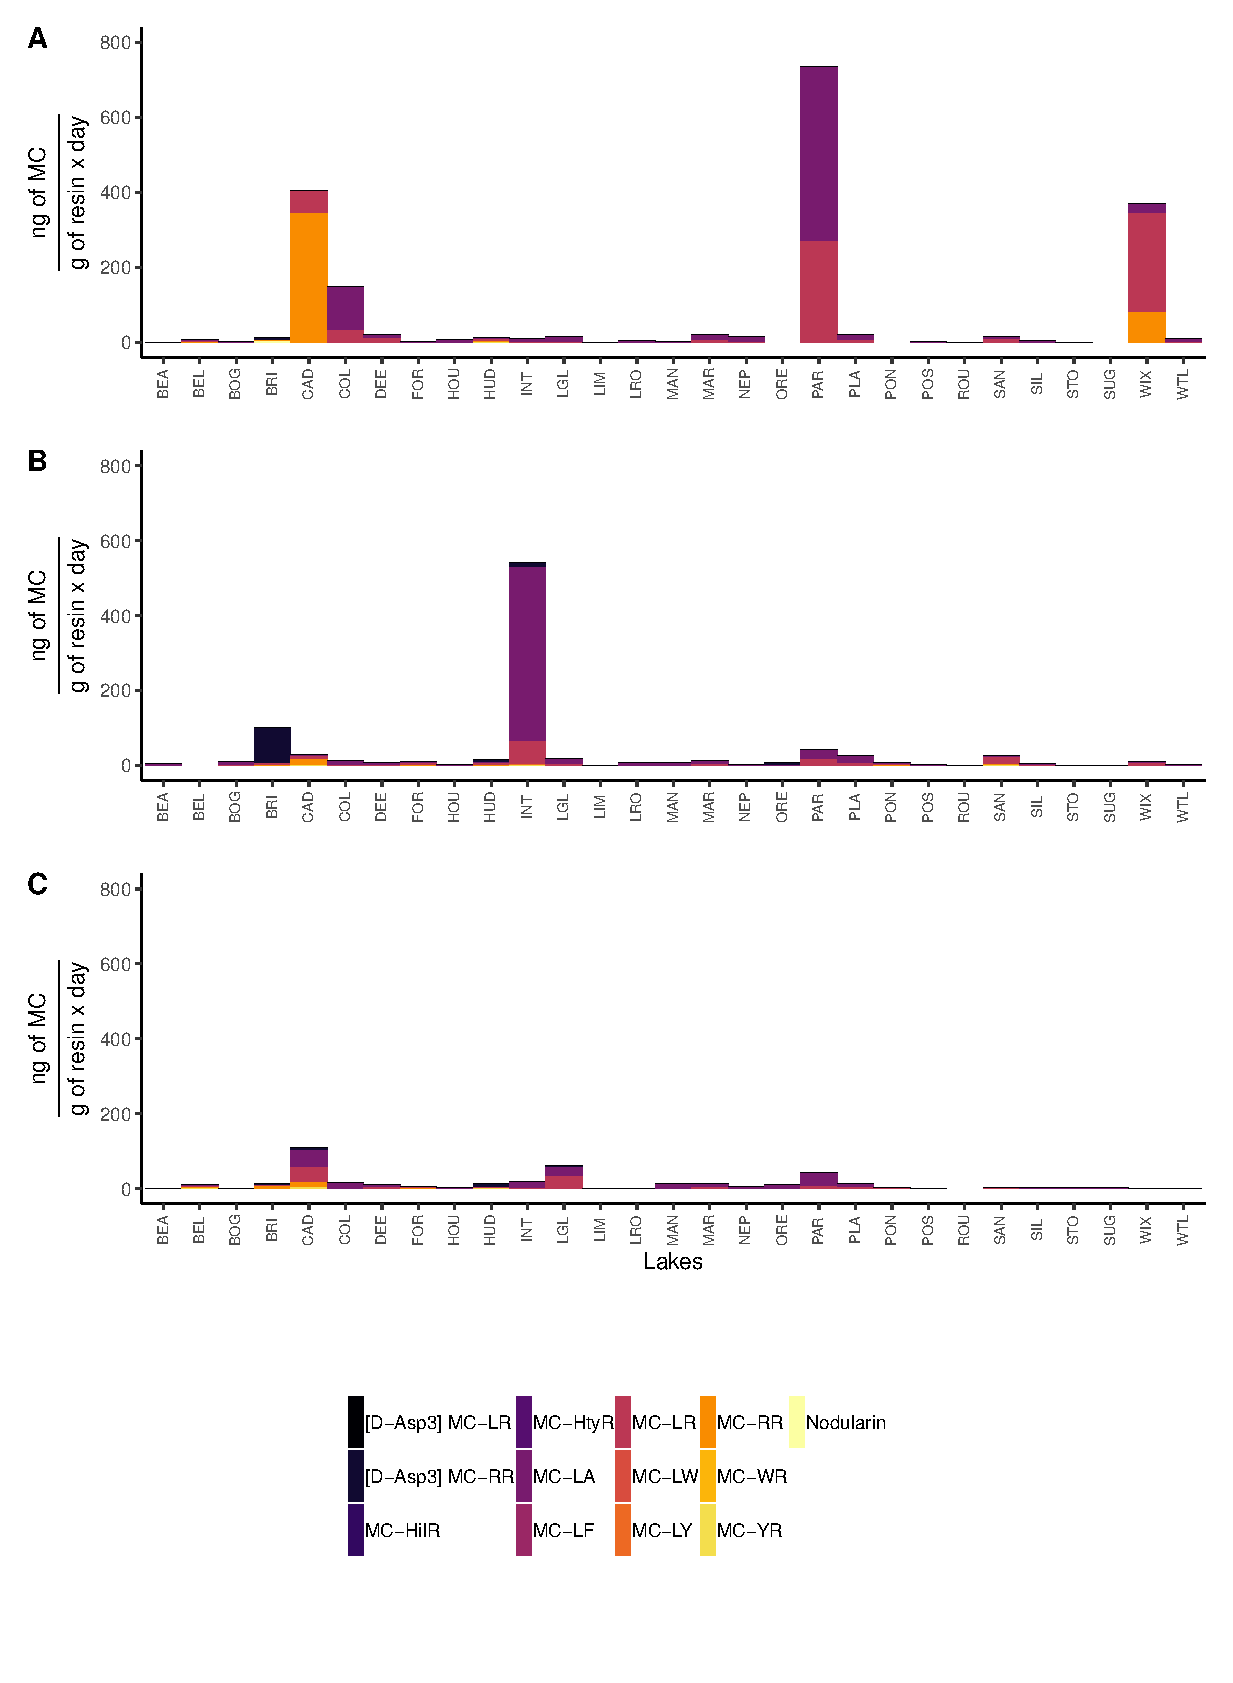
\includegraphics[width=\textwidth]{figures/spatter}
	\caption{TODO}
	\label{fig:spatter}
\end{figure}

\clearpage




\section{Statistical Modeling}
\subsection{Exploratory Analysis}

With our model selection, a correlation matrix analysis was done to observe any possible collinear relationships between our predictor variables. The correlation matrix analysis showing only significant relationships and arranged by the anglular order of eigenvectors and identified few correlated variables  (see \ref{matrix}, and see \ref{fig:matrixfull} for the full correlation values). In our correlation matrix analysis, we observed a few relationships that may be meaningful. We found turbidity positively correlated with orthophosphate, total phosphorus, total Kejldahl nitrogen, water temperature, phycocyaninin and chloraphyll. Chlorophyll is positively correlated with \emph{mcye}, phycocyanin, \emph{16S rRNA}, total Kejldahl nitrogen and orthophosphate. Conductance was found to have negative relationship with precipitation.
Developed land-use is positively correlated with nitrate+nitrite, total nitrogen and conductance.
Watershed area was positive correlated with Zebra mussel mass.
Agriculture had a positive relationship with nitrate+nitrite,
Forest land-use had negative correlation with total Kejldahl nitrogen, total nitrogen, conductivity, ammonia, nitrate+nitrite and total nitrogen to total phosphorus ratio.
Precipitation had negative correlation with total nitrogen, orthophosphate and conductivity.

From our best subset analysis with the largest subset size of 3 (nvmax=3),  orthophosphate, \emph{mcyE}, turbidity, max depth,  lake area to watershed ratio, barren land-use and precipitation 3 days prior to sampling were frequently chosen  predictor variables for MC concentration (see figure \ref{subset}).


%Proper way to assess collinearity by linear regression? A caused by B and B caused by A?
From our data, $log10$(Orthophosphate) was shown to be positively correlated with $log10$(turbidity) from our exploratory analysis, with a simple linear regression analysis, the relationship is slightly significant ($\beta=0.57$, $F_{{1,26}}=3.13$, $p=0.08$). The regression did have outliers, with the two data points removed the relationship is significant ($\beta=0.17$, $F_{{1,25}}$, $p=0.01$) (see \ref{fig:plot1}). We avoid including either $log10$(orthophosphate) or $log10$(turbidity) in our models together.
%All other variables did not have any significant correlations with eachother.
%From backward stepwise regression, eliminated  contained 3 variables, orthophosphate, max depth and turbidity.
With $log10$(\emph{mcyE}) as a single predictor in a linear mixed model shown to have a significant relationship with $log10$(MC), however we are missing data from July ($N=91$) which does not allow us to use the full dataset ($\beta=0.15$, $F_{{1,72}}$, $p=0.002$).

We found $log10$(turbidity) as the best single predictor. The relationship was significant with predicting $log9$(MC) concentration in a linear mixed-effect model ($\beta=0.55$, $F_{{1,27}}=5.90$, $p=0.02$) (see \ref{fig:plot2}). However, with $log10$(orthophosphate) as a single predictor the relationship is almost significant ($\beta=0.35$, $F_{{1,26}}=3.13$, $p=0.07$) (see \ref{fig:plot2}).  The best model for predicting MC is turbidity as the sole predictor. Adding additional predictors did not significantly improve the model.

For predicting the $log10$(\emph{16s rRNA}) gene copies, chloraphyll, agriculture land-use and average temperature 3 and 30 days prior to sampling and precipitation 5 days before sampling were investigated for building our model (see figure \ref{subset2}). Precipitation and temperature data did not have significant relationship and was eliminated from the model. Agriculture percent land-use found to be the best predictor for \emph{16s rRNA} ($\beta=0.70$, $F_{{1,26}}=5.10$, $p=0.03$)(figure \ref{fig:agriculture})



\subsection{\emph{A Priori} Hypothesis Test}

In my hypothesis, I expected developed land-use percentage to have a positive influence on MC concentrations. Much of the southern lakes were vastly dominated by developed land such as Belleville, Ore, Brighton, Ford and Bogie Lake. 
Developed land-use percentage plotted had a slight positive effect with $log10$(MC) concentration , however the relationship was not significant  ($\beta=0.59$, $F_{{1,27}}=1.75$ , $p=0.20$)(see figure \ref{fig:developed}) . There were no significant relationship with developed land-use percentage in predicting $log10$(\emph{16s rRNA}) gene copies ($\beta=0.48$, $F_{{1,25}}=1.75$ , $p=0.27$). However, developed land-use had a positive significant relationship with log10(nitrate+nitrite) ($\beta=0.75$, $F_{{1,27}}=1.08$, $p=0.018$)

Forest land-use percentage had a significant negative relationship with $log10$(\emph{16s rRNA}) gene copies ($\beta=-1.42$, $F_{{1,25}}=7.08$, $p=0.013$)(see figure \ref{fig:forest}). Albiet, forest land use did not have a significant effect on $log10$(MC) concentrations ($\beta=-0.34$, $F_{{1,26}}=0.32$, $p=0.57$).

With the surveyed lakes, 17 out of 29 had Zebra mussels found in the month of October. The average MC concentrations with  of Zebra mussles present was 0.568 $\mu$g/L, and absent with 0.305 $\mu$g/L. Using a two sample Student's t-test, we fail to reject the null where difference of the mean is greater than 0 ($t=1.14$, $df=107$, $p=0.13$). We also did not find any significant relationship with the mussel counts and mass with predicting MC concentration.



\begin{sidewaysfigure}[!hp]

  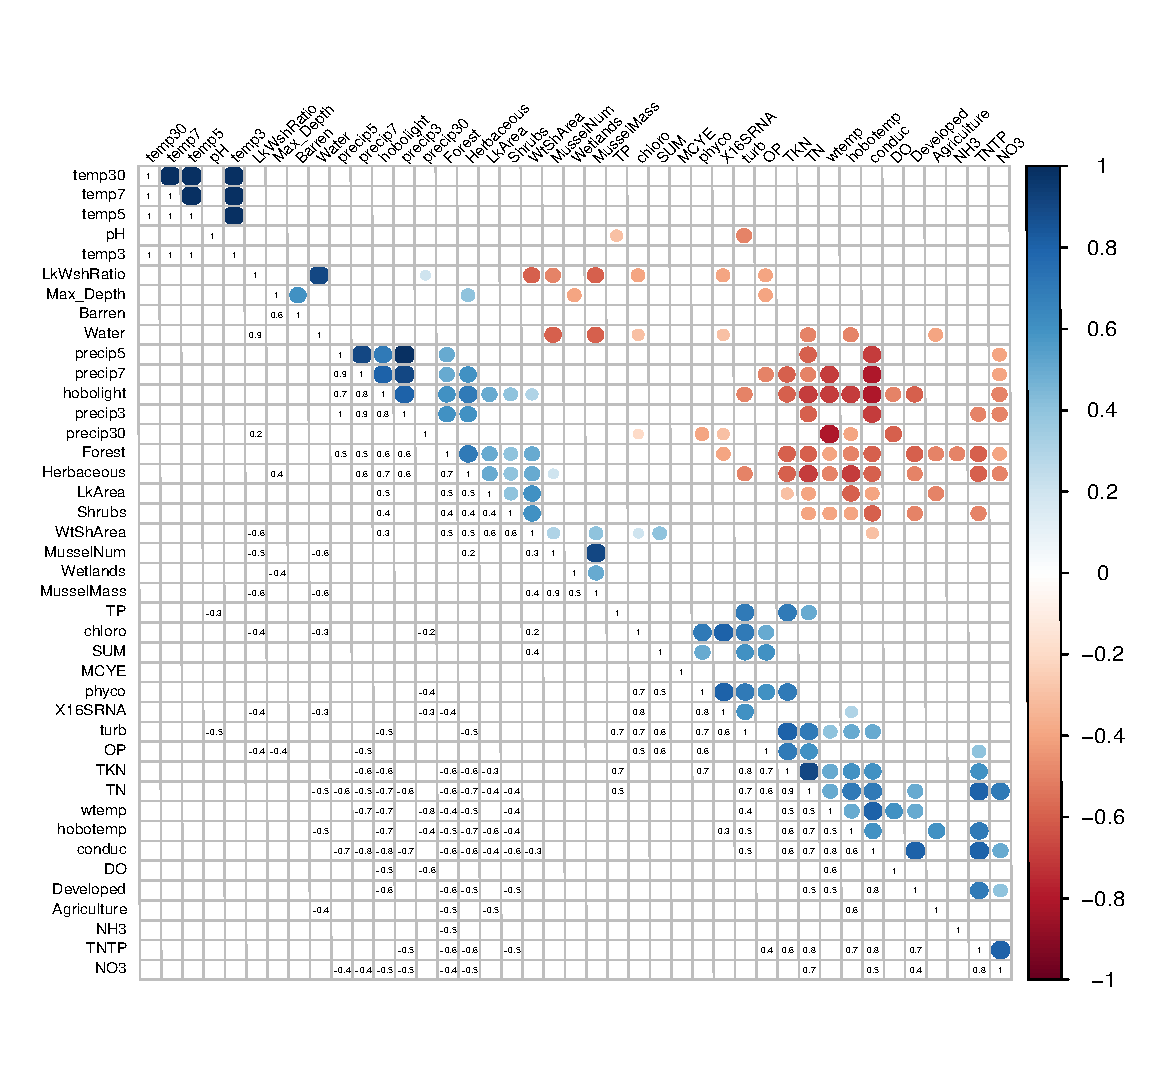
\includegraphics[width=0.7\textwidth]{matrix}
  \vspace*{-10mm}
  \caption{
  Correlation matrix with calculated Pearson coefficient in the lower triangle, and a graphical representation of coefficient value in the upper triangle. Each pair was tested for association between paired variables with Pearson's product moment correlation with relationships not shown if $\alpha>0.05$. Data matrix was arranged by the angular order of the eigenvectors.}
  \label{matrix}
\end{sidewaysfigure}


\begin{figure}[!ht]
  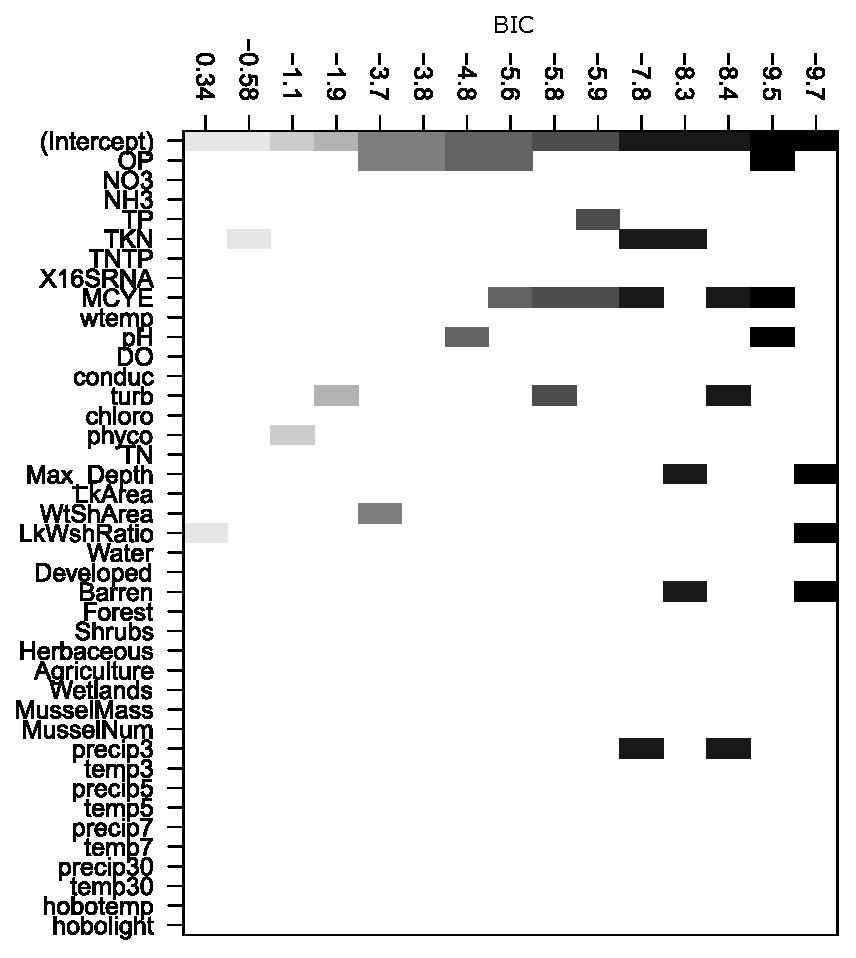
\includegraphics[angle=90,height=8cm, width=\textwidth]{Subset}
  \caption{Subset regression analysis with MC Sum from LC-MS/MS as response variable. Each row is a model. Variable is included in the model it is represented as a black rectangle. The BIC is plotted on the y axis where the lowest value is higher up on the axis.}
  \label{subset}
\end{figure}

\begin{figure}
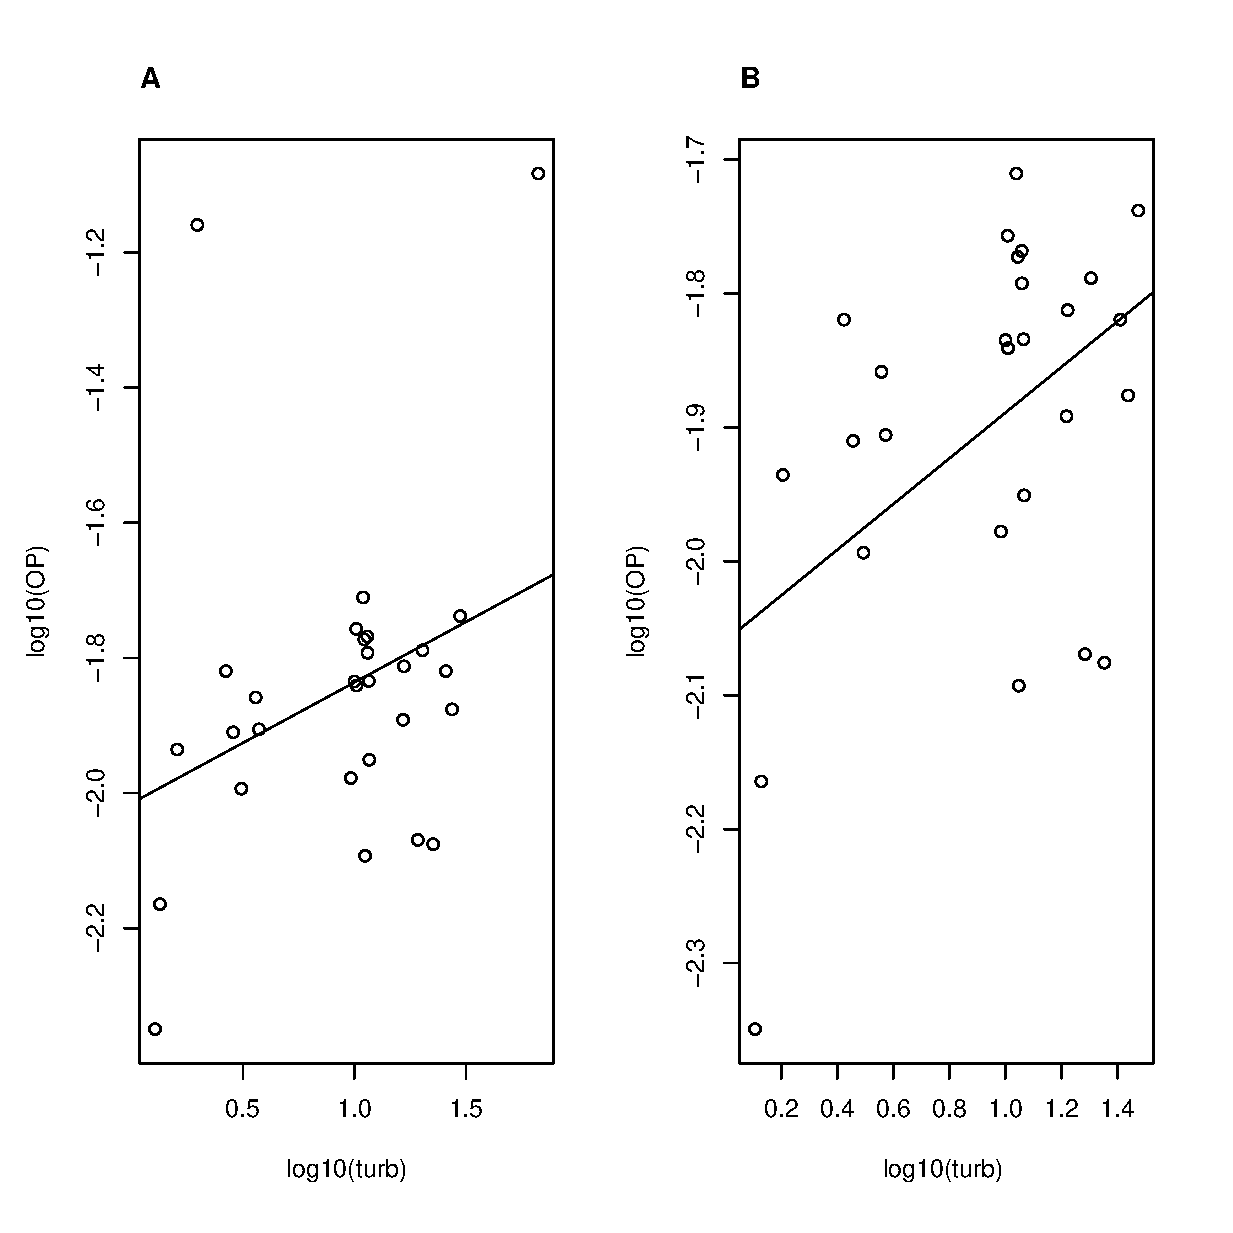
\includegraphics[width=\textwidth, height=11cm]{figures/plot1}
\caption{
(A): Positive relationship with average $log10$(OP) with average $log10(turb)$ ($\beta=0.57$, $F_{{1,26}}=3.13$, $p=0.08$).
(B): With two outliers removed, the relationship between $log10(OP)$ and $log10(turb)$ was signifigant  ($\beta=0.17$, $F_{{1,25}}$, $p=0.01$).
}
\label{fig:plot1}
\end{figure}

\begin{figure}
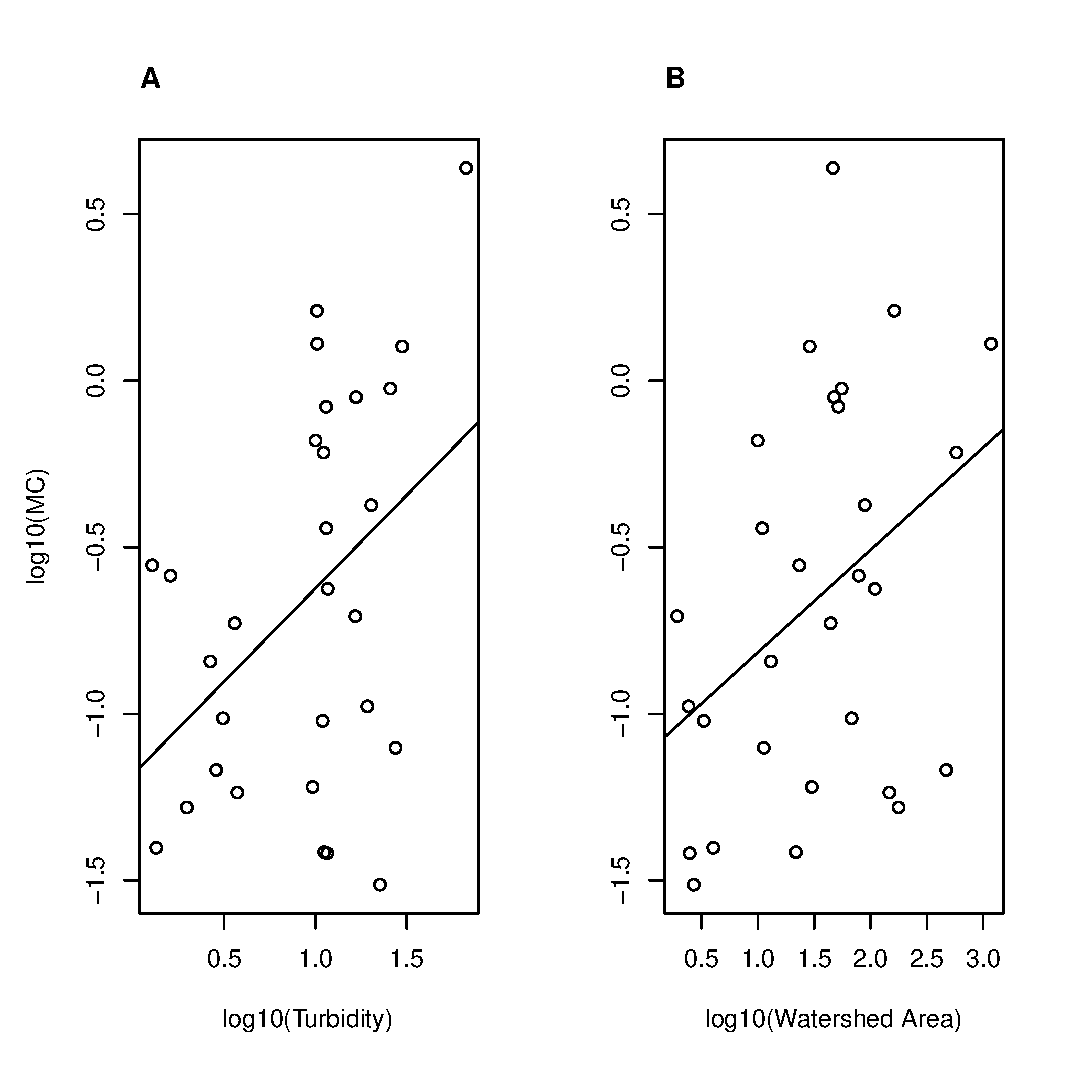
\includegraphics[width=\textwidth, height=11cm]{figures/plot2}
\caption{
(A): Positive relationship between average $log10$(MC) with average $log10(turb)$ ($\beta=0.55$, $F_{{1,27}}=5.90$, $p=0.02$)
(B): Positive relationship between average $log10(MC)$ and average  $log10$(OP) ($\beta=0.35$, $F_{{1,26}}=3.13$, $p=0.07$). 
Turbidity is our best predictor variable for MC. Orthophosphate is nearly significant predictor}
\label{fig:plot2}
\end{figure}

\begin{figure}[!ht]
  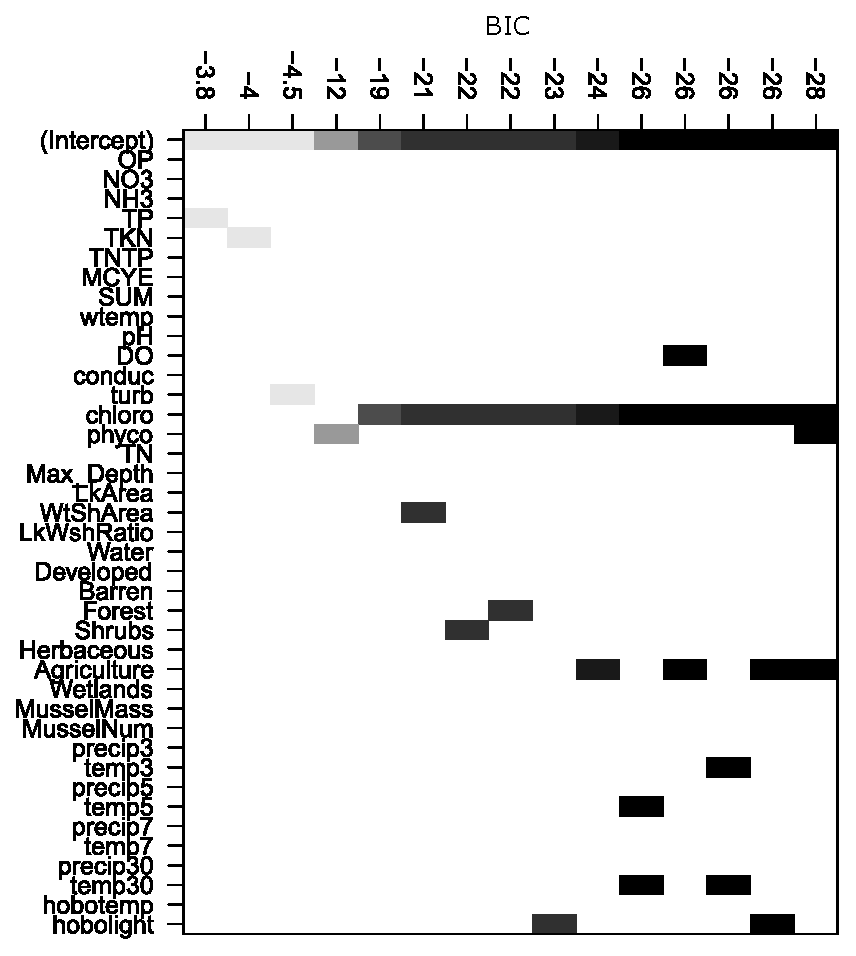
\includegraphics[angle=90,height=8cm, width=\textwidth]{Subset1}
  \caption{Best Subset: \emph{16s rRNA} Gene copies as response variable}
  \label{subset2}
\end{figure}




\begin{figure}
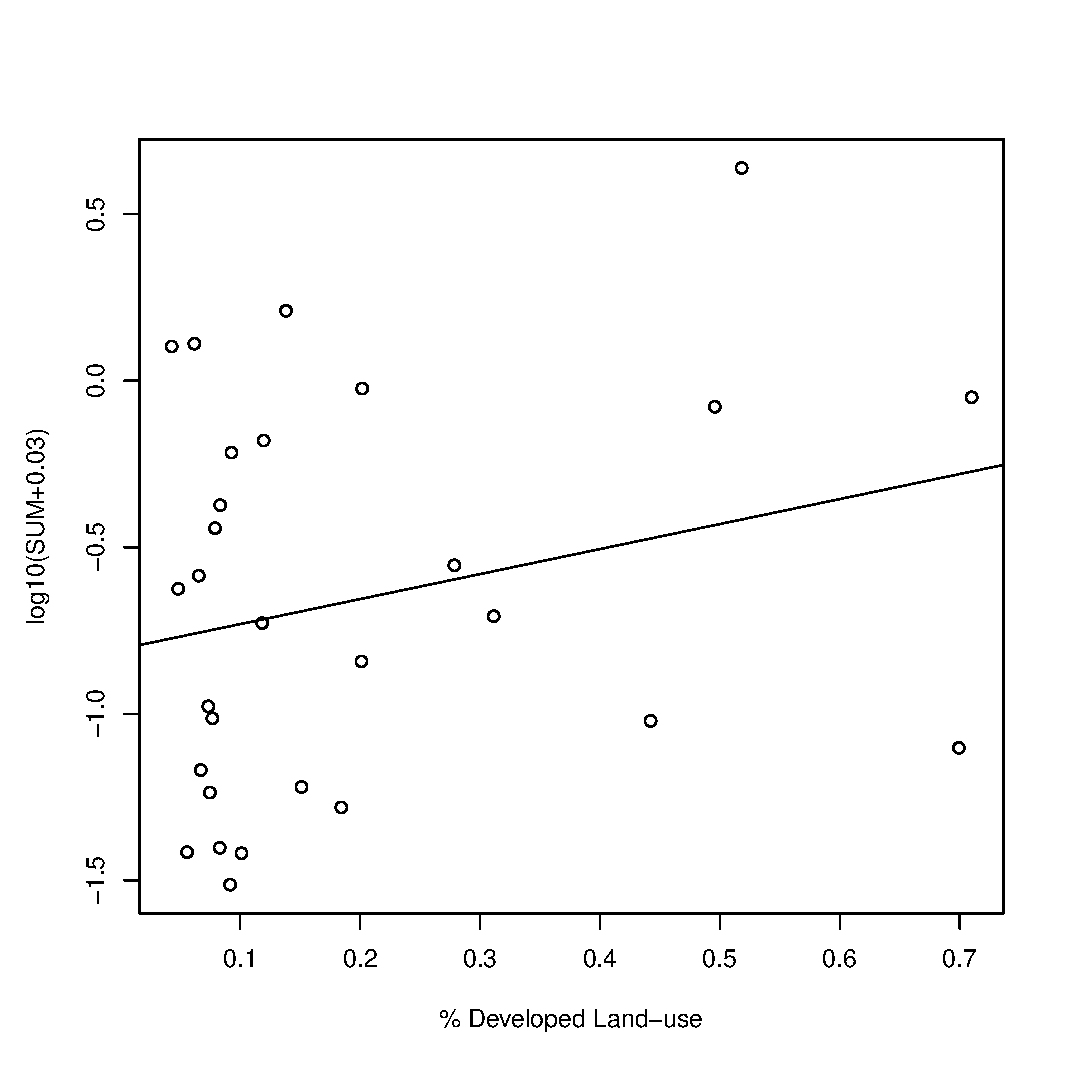
\includegraphics[width=\textwidth]{figures/developed}
\caption{A slight positive relationship between $log10(MC)$ and developed land use. ($\beta=-0.59$, $F_{{1,27}}=1.75$, $p=0.20$)}
\label{fig:developed}
\end{figure}

\begin{figure}
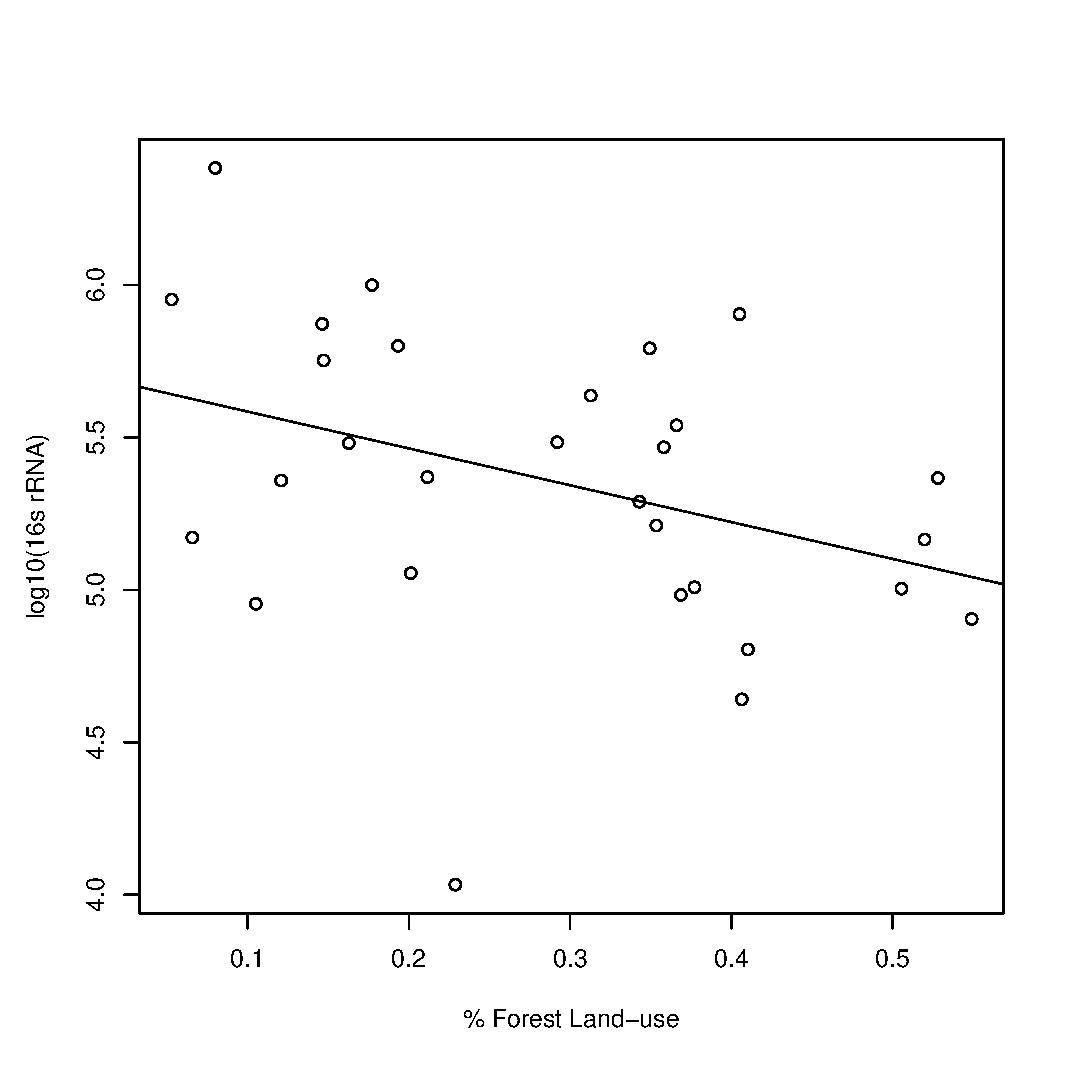
\includegraphics[width=\textwidth]{figures/forest}
\caption{A negative relationship between $log10(MC)$ and forest land use. ($\beta=-1.42$, $F_{{1,25}}=7.08$, $p=0.013$)}
\label{fig:forest}
\end{figure}




\begin{figure}[!ht]
  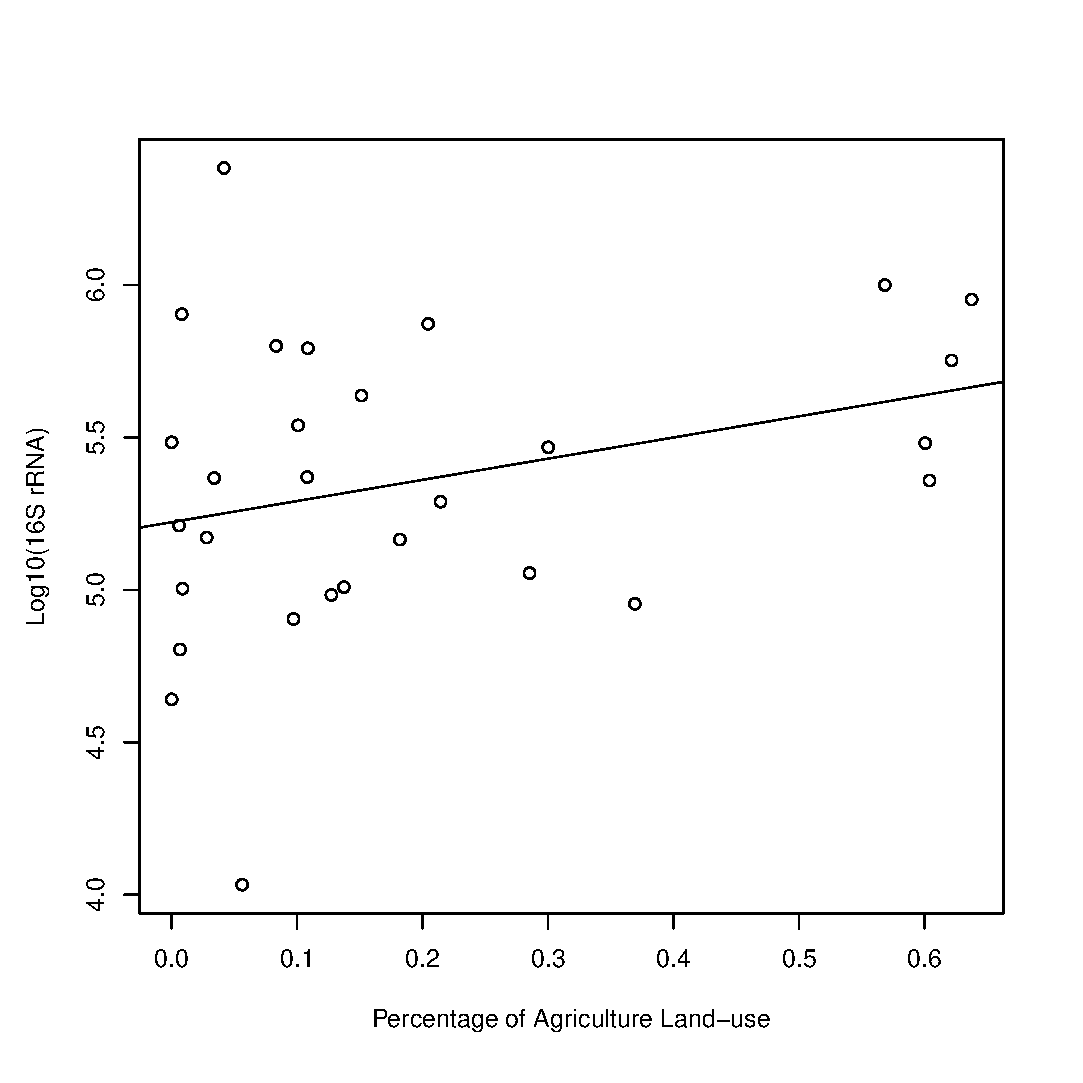
\includegraphics[width=\textwidth]{figures/Agriculture}
  \caption{Positive relationship between percent agriculture land-use and $log10$(\emph{16s rRNA}) ($\beta=0.70$, $F_{{1,26}}=5.10$, $p=0.03$)}
  \label{fig:agriculture}
\end{figure}
\clearpage



\section{Discussions}

When \gls{lcmsms} and ELISA are compared in our grab samples, there are discprenancies between the two. Analysis from ELISA tends to be report higher values than \gls{lcmsms}. The difference is more apparent in the month of September and October, where the difference can be quite large (see figure \ref{fig:compare}). The ELISA generally presents a higher result than \gls{lcmsms}. This is in part due to the detection limit and reportable limits being much higher for the ELISA, 0.15 and 0.1 $\mu$g/L. However, our analysis in the month of August had good agreement between \gls{lcmsms} and ELISA.  

\begin{figure}[!h]
	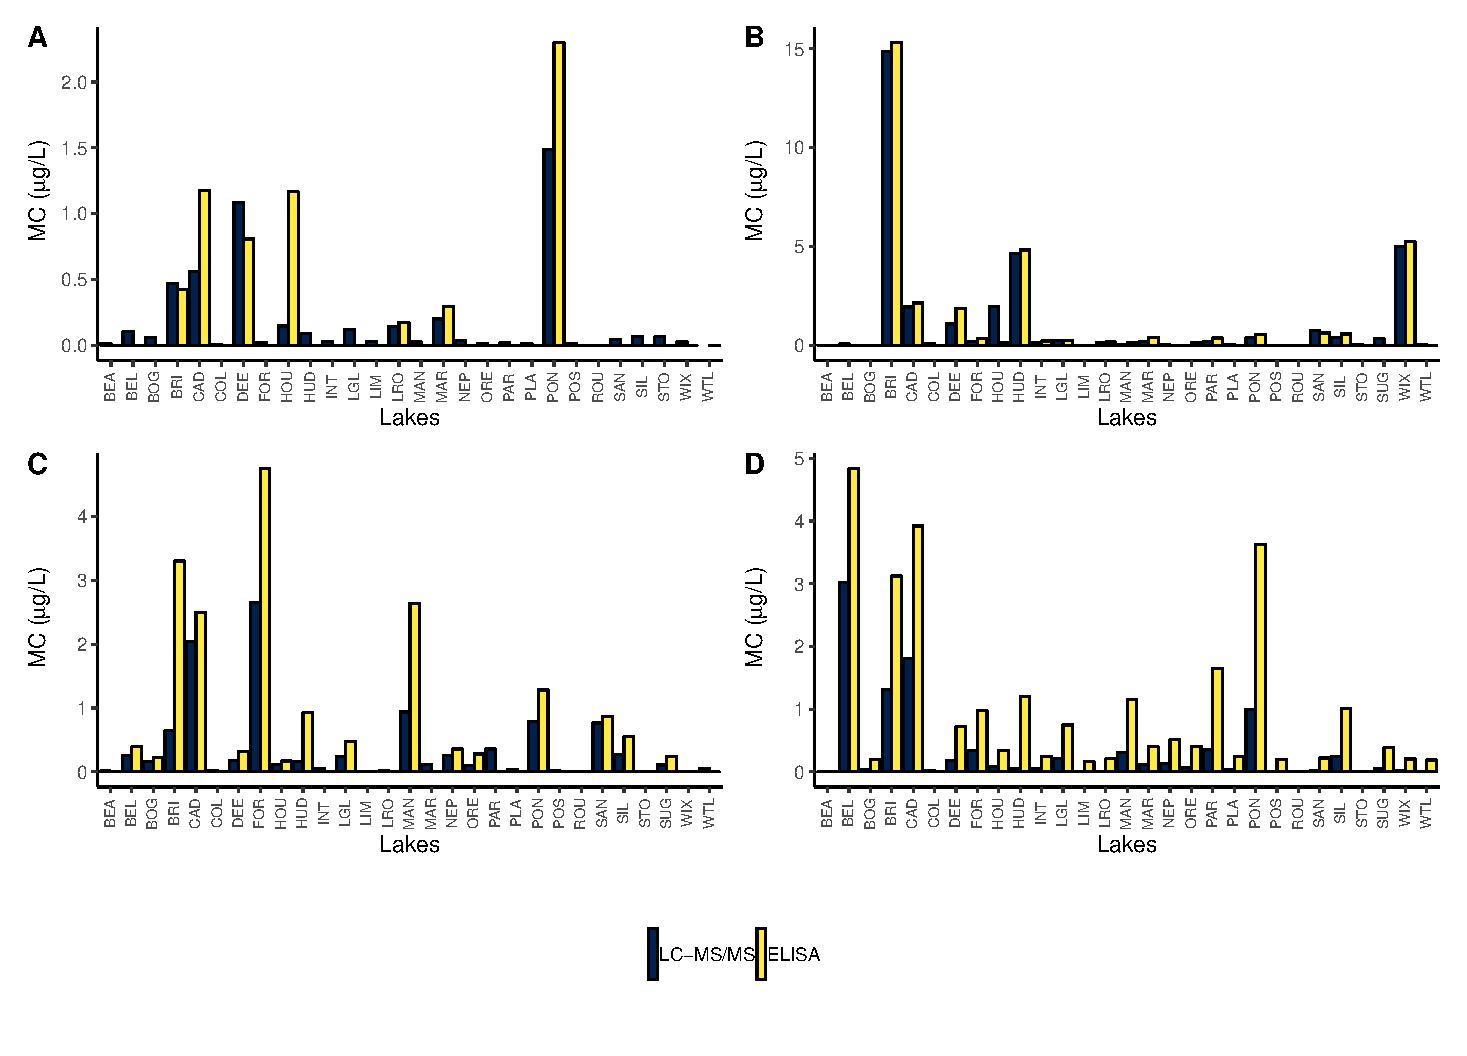
\includegraphics[width=\textwidth]{figures/compare}
	\caption{TODO}
	\label{fig:compare}
\end{figure}

% Comparing the results between MC concentrations and \emph{16s rRNA}, we can see a difference in figure \ref{fig:resbar}.
% Lake turnover, winter stable, spring mix, summer stable, fall mix. 
% Microcystin concentration tells a different story compared to \emph{16s rRNA}. This curve is to be expected due to warmer temperature as our data does follow this pattern (see figure \ref{fig:hobo}).

In our first hypothesis, I tested if disturbance from developed land is associated with \gls{hab} and if it has an affect on nutrient concentration.  From our data, we did not find a significant relationship between developed land use and MC concentrations or \emph{16s rRNA}. However, we did find developed land use having some effect with nitrate+nitrite.

Forest has negative correlation with NUTRIENTS

Disturbances of flora contributes to lower nutrient retention and hydrological impacts that can cause more blooms \cite{anderson_harmful_2002, codd_cyanobacterial_2000, fraterrigo_influence_2008}.
\gls{mc} could increase as developed is more prevalent in the lake's watershed.


Orthophosphate was shown to be slightly signifigant. The bioavailability of phosphorus is pH dependent, where most is available between when in alkaline conditions with a pH>8 \cite{lucas_relationships_1961}.
Mostly all of our sampled lakes were mostly alkaline conditions averaging around 8.53$\pm$0.37 pH ranging from 7.44 to 9.94. Lakes that had levels above the health advisory levels did have pH that were above 8. Lake Paradise, Brighton %%% REVISE THIS TODO

Wixom lake is very unique, it has the largest watershed amongst all our surveyed lake and has visually one of the largest extent


%Dissolved oxygen averaged around 12.98$\pm$20.8 mg/L of \ch{O2}.

% FORMS OF NUTRIENTS TODO revise this, expand it
In controlled lab experiments, nutrients such as inorganic nitrogen or phosphorus are found to be limiting growth factors. In a  when \emph{Microcystis aereginosa} grown in the laboratory \cite{xiao_colony_2018, yema_role_2016}.

% revise this and put more work into this TODO
Cyanobacteria are versatile as they can acquire nutrients under extreme conditions. They can utilize a process called quorom sensing which they coordinate with each other by using a signaling hormone acylated homoserine lactones \cite{van_mooy_quorum_2012}. They also can create a network of cells which work together as a unit, often as seen as a layer of green goo floating on top of water.  There are very robust organisms, as some can change their buoyancy by modulating the intracellular gas vesicles gives them a competitive advantage over other species for seeking light \cite{feng_how_2018}.\emph{Microcystis} can form a complex colony made by a mucilage structure which can be bouyant due to high concentration of dissolved oxygen \cite{xiao_colony_2018}. % TODO expand how co2 gets pumped into gas vesicles
Most of the cyanotoxin are intracellular, however with increase turbulence from wind and precipitation can release more toxins due to cell lysis either from cell apoptosis or from mechanical abruption which release \cite{rohrlack_fate_2007}. % TODO cyanophages, viruses 



%A study in South Korea found 3-week lagged water temperature,dissolved oxygen and pH with to correlate with each other in their models \cite{ahn_evaluation_2011}.

%Growing cyanobacteria measurements taken at the same time . Their is an assumption being made.

%Total nitrogen was found to explain the variance of MC concentrations \cite{taranu_predicting_2017}.

%Man-made lakes are found to be twice as higher concentrations in cylindrospermonsin \cite{loftin_cyanotoxins_2016}.


%Low-nutrient lakes can still exhibit blooms.
 %This can complicate our model as this is not accounted for.

%QPCR results as a response variable comes with complication as this does not distinguish alive or dead cyanobacteria.




%Water sampling for nutrient is difficult. Time series data, nutrient dynamic. Continuous measurements  water data would be best, but for a large survey its almost impractical. Other organisms compete with these common nutrients. Aquatic macrophytes largely acquire dissolved phosphorus. Time between sampling the lake at the peak of the bloom and the flush of nutrient inputs can be lagged, and most likely different depending on each lakes morphology. Biological properties are not necessarily linear. One thing to consider here is the sampling frequency. We sampled once a month for four months, which gives four sampling results for each lake. This may not explain everything about each lake.

% How pH and DO has an influence on nutrient availability

Comparing the average results from SPATT to the grab sample, we identified a major difference (see \ref{fig:spattbox}). When average concentration of MC from SPATT and grab sample is ordered by latitude, we found the relative mangitude of microcystin is higher found in the upper latitude of Michigan compared to regular grab sample. In our grab sample, Brighton, Pontiac, Wixom Lake and Lake Cadillac had high average MC with notable \gls{hab}.

The results from SPATT seemed to suggest the lakes we found to have low microcystin from our grab sample missed other \gls{hab}. When lakes were ordered by latitude, it also suggest lakes found in the upper latitude of Michigan may had higher frequency of \gls{hab}.

We suggest there is another factor that explains the higher magnitude of microcystin. We started to observe biofilm to accumulate on the SPATT bags. The biofilm was more notable in lakes that had significant blooms such as Brighton, Pontiac, and Wixom Lake. Initially we did not expect this would effect the capacity of the SPATT, but this data may suggest this. In our next year of survey we will test the hypothesis if the biofilm has a negative effect of microcystin adsorption. We may need to dispatch the SPATT bags more often to prevent biofilm to encase and clog the Nitex mesh bag.

\begin{figure}[!hp]
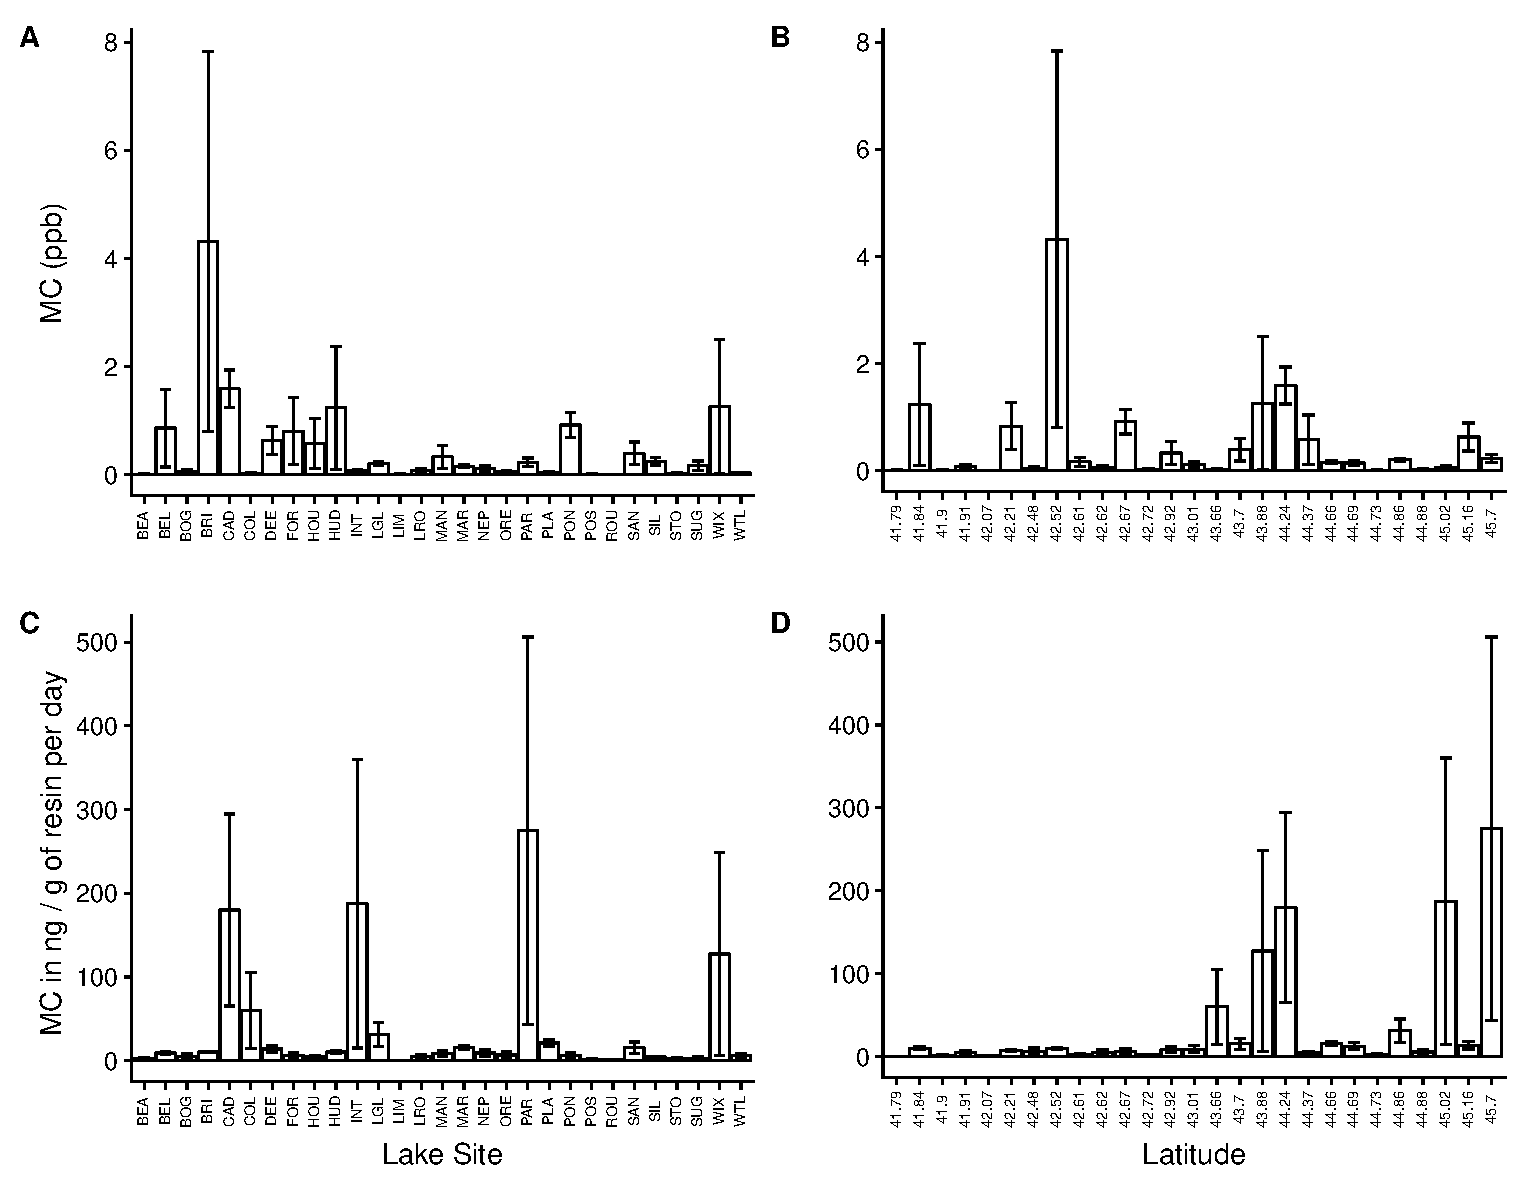
\includegraphics[width=\textwidth]{figures/spatttboxplotlake}
\caption{
Microcystin measured from SPATTS compared to grab sample: and Grab Samples. Average concentration of MC are plotted as bar graphs. Microcystin concentrations analyzed from grab sample are shown in figure (A) arranged by each lake and (B) arranged by latitude. Microcystin concentrations analyzed from SPATT samples are shown in figure (C) arranged by each lake and figure (D) arranged by latitude
}
\label{fig:spattbox}
\end{figure}







